%% tex/timespacehierarchies.tex
%% Copyright 2019 Andrea Berlingieri
%
% This work may be distributed and/or modified under the
% conditions of the LaTeX Project Public License, either version 1.3
% of this license or (at your option) any later version.
% The latest version of this license is in
%   http://www.latex-project.org/lppl.txt
% and version 1.3 or later is part of all distributions of LaTeX
% version 2005/12/01 or later.
%
% This work has the LPPL maintenance status `maintained'.
%
% The Current Maintainer of this work is Andrea Berlingieri.
%
% This work consists of all files listed in manifest.txt
\chapter{Gerarchie in spazio e tempo}

%Slide 73

\section{I teoremi della gerarchia}

I teoremi che seguono sono tra i più importanti della teoria della calcolabilità. Riflettono
l'idea intuitiva che disponendo di una quantità maggiore di risorse è effettivamente possibile
affrontare problemi più complessi.

Consideriamo $\DTIME(n^{2})$, ovvero la classe dei linguaggi riconoscibili in tempo quadratico e
$\DTIME(n^{3})$. Qual'è la relazione di inclusione tra queste due classi? Abbiamo sicuramente che
$\DTIME(n^{2}) \subseteq \DTIME(n^{3})$.

In generale abbiamo che, se $f,f'$ sono funzioni da $\Nat$ a $\Nat$:
\begin{equation*}
    O(f) \subseteq O(f') \implies \DTIME(f) \subseteq \DTIME(f')
\end{equation*}
Vale lo stesso per lo spazio. Ricordiamo che $O(f) \subseteq O(f') \iff f \in O(f')$.

Ci chiediamo ora, questa inclusione è stretta? E sotto che ipotesi possiamo affermare ciò?
Esistono, ad esempio, dei linguaggi riconoscibili in tempo $O(n^{3})$ ma non in tempo $O(n^{2})$? E
analogamente per lo spazio?

La risposta è, in un certo senso, positiva, sia per tempo che spazio. Vale più per lo spazio che
per il tempo, poichè lo spazio è più ``grezzo'' del tempo come misura. La separazione in classi
risulta più difficile con una misura fine come quella del tempo.

\subsection{Il teorema della gerarchia in spazio}

Vediamo innanzitutto come formalizzare il teorema ponendo la nostra attenzione sullo spazio.  Stiamo
facendo il confronto tra $\DSPACE(n^{2})$ e $\DSPACE(n^{3})$. Quello che vogliamo concludere è che
dato che $n^{3} \notin o(n^{2})$, allora $\DSPACE(n^{3}) \not\subseteq \DSPACE(n^{2})$. Da cui si
ottiene, data l'inclusione precedente, $\DSPACE(n^{2}) \subset \DSPACE(n^{3})$.

\begin{thm}
    Siano $f,f':\Nat \to \Nat$. Si ha che:
    \begin{equation*}
        f \in O(f') \implies \DSPACE(f) \subset \DSPACE(f')
    \end{equation*}
\end{thm}

Per dimostrare il teorema, dando per ovvia l'inclusione non stretta, ci è sufficiente dimostrare
che:
\begin{equation*}
    f \notin O(f') \implies \DSPACE(f) \not\subseteq \DSPACE(f')
\end{equation*}

Il teorema in questa forma è dimostrabile. Esiste tuttavia una forma più debole ma più intuitiva:
\begin{equation*}
    f' \in o(f) \implies \exists \Lang, \Lang \in \DSPACE(f) \land \Lang \notin \DSPACE(f')
\end{equation*}
Abbiamo rafforzato la premessa dell'implicazione e quindi indebolito il teorema. Ricordiamo che $f'
\in o(f) \implies f \notin O(f')$.

È uno dei pochi teoremi della teoria della complessità che ci permettono di separare nettamente
classi di complessità. Questo è in contrasto con le tante inclusioni congetturate che non
riusciamo a dimostrare, la più famosa delle quali è la questione $\PClass$  vs $\NPClass$.

\begin{proof}
    Questo teorema è sicuramente intuitivo nell'enunciato ma non è ovvio nella dimostrazione.

    Per dimostrare il teorema dobbiamo, sotto l'ipotesi $f' \in o(f)$, definire il nostro linguaggio
    $\Lang$ e poi dimostrare le proprietà attese per $\Lang$.

    %Ce ne sono diverse di dimostrazioni di questo teorema (sul Sipser ce ne è una diversa). La
    %dimostrazione non è banale, va studiata e capita. È utile farsi guidare dall'enunciato.

    La tecnica tipica che si usa quando si vuole creare un elemento che non faccia parte di una
    certa classe è la diagonalizzazione. In questo caso definiamo il nostro $\Lang$ per
    diagonalizzazione in modo che non sia riconoscibile in spazio $O(f')$.

    Vediamo prima una versione sbagliata del linguaggio, per poi passare a quella corretta. Questo
    passaggio ci porterà a capire una cosa importante della complessità.

    Usiamo la notazione $\code{M}$ per denotare il codice della MdT $M$.

    Definiamo $\Lang$ come:
    \begin{equation*}
        \Lang = \set{\code{M} \mid \code{M} \notin \Lang_{M} \land s_{M}(|\code{M}|) \leq f(|\code{M}|)}
    \end{equation*}

    La seconda parte della congiunzione ci garantisce che la complessità in spazio delle macchine
    il cui codice fa parte di $\Lang$ su stringhe di lunghezza $|\code{M}|$ sia $O(f)$.

    Procediamo per contraddizione. Supponiamo che $\Lang \in \DSPACE(f')$. Ovvero, $\exists M_{0}$ tale
    che $\Lang_{M_{0}} = \Lang$ e inoltre $M_{0}$ lavora in spazio $O(f')$.

    Ci chiediamo ora, $\code{M_{0}} \in \Lang$? Questo è vero sse $\code{M_{0}} \in \Lang_{M_{0}}$.
    Dalla definizione di $\Lang$ abbiamo $\code{M_{0}} \notin \Lang_{M_{0}} \land
    s_{M_{0}}(|\code{M_{0}}|) \leq f(|\code{M_{0}}|)$. 

    Abbiamo quindi:
    \begin{equation*}
        \code{M_{0}} \in \Lang \iff \code{M_{0}} \notin \Lang_{M_{0}} \land s_{M_{0}}(|\code{M_{0}}|)
        \leq f(|\code{M_{0}}|)
    \end{equation*}

    Abbiamo che la prima parte del $\iff$ è incompatibile con la prima parte della congiunzione.
    Per avere una contraddizione dobbiamo fare in modo che la seconda parte della congiunzione
    risulti vera.

    Ci bastano le ipotesi che $M_{0}$ lavora in spazio $O(f')$ e che $f' \in o(f)$ per affermare
    che, su input $\code{M_{0}}$, avremo che $M_{0}$ lavorerà in spazio al più limitato da
    $f(|\code{M_{0}}|)$? La risposta è no, poichè quando parliamo di complessità computazionale
    parliamo di complessità asintotica, mentre qui ci stiamo chiedendo quale sia il comportamento
    della funzione in un punto particolare. $\code{M_{0}}$ potrebbe essere un punto sfortunato, come
    mostrato in figura \ref{img:spacehierarchy}.

    La complessità asintotica non ci dice niente su cosa succede su un determinato input.

    Come procediamo? In questo caso il problema non è particolarmente complicato. Siccome sappiamo
    che la complessità asintotica della macchina $M_{0}$ sarà più bassa di $f$ dobbiamo
    ``spostare'' l'input un pò più in là, per essere certi del comportamento di $M_{0}$ in quel
    punto. Per fare ciò andiamo a rivedere la definizione del linguaggio $\Lang$.
    \begin{equation*}
        \Lang = \set{\pair{\code{M}}{x} \mid \pair{\code{M}}{x} \notin \Lang_{M} \land
        s_{M}(|\pair{\code{M}}{x}|) \leq f(|\pair{\code{M}}{x}|)}
    \end{equation*}

    La $x$ è una stringa aggiuntiva che non fa altro che accrescere la dimensione dell'input.

    Come prima, supponiamo che $\Lang \in \DSPACE(f')$, con macchina $M_{0}$ che riconosce $\Lang$ e
    lavora in tempo $O(f')$. Sappiamo che $f' \in o(f)$, ovvero esiste un punto $m$ tale che, per
    valori in input maggiori di $m$, abbiamo che $f'$ sta definitivamente al di sotto di $f$.
    Scegliamo ora un $x_{0}$ la cui rappresentazione in memoria ha una dimensione maggiore di $m$.
    Avremo sicuramente che $f'(|x_{0}|) < f(|x_{0}|)$, e questo varrà maggiormente per stringhe con
    una dimensione maggiore di quella di $x_{0}$.

    \begin{figure}[h]
        \begin{center}
            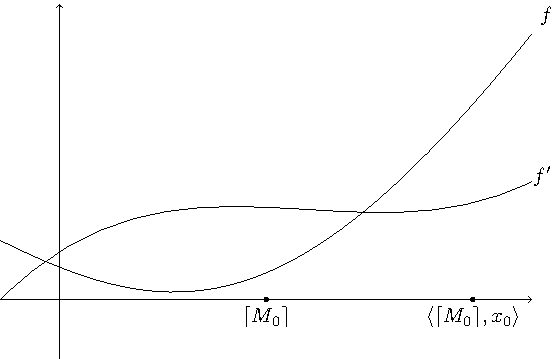
\includegraphics{./img/timespacehierarchies/spacehierarchy.pdf}
            \caption{L'input $\code{M_{0}}$ potrebbe essere in una posizione sfortunata. In generale
            non possiamo fare assunzioni su dove si trovi. La soluzione è usare un $x$ che sposti
            più in là l'input, dove abbiamo la certezza che $f$ sia al di sopra di $f'$}
            \label{img:spacehierarchy}
        \end{center}
    \end{figure}

    Quello che vogliamo è quindi spostare l'input in un punto tale che da lì in poi $f$ sarà
    definitivamente al di sopra di $f'$. Di fatto noi siamo interessati alla complessità della
    macchina $M_{0}$, ma sapendo che questa lavora in spazio $O(f')$ avremo che dal punto che
    raggiungiamo con il ``padding'' dato da $x_{0}$ in poi questa lavorerà in uno spazio che sarà
    definitivamente minore di $f$ a meno di una costante.

    %(Sulla registrazione c'è la spiegazione della validità di questo claim).
    Ci chiediamo ora se $\pair{\code{M_{0}}}{x_{0}} \in \Lang$. Questo succede sse
    $\pair{\code{M_{0}}}{x_{0}} \in \Lang_{M_{0}}$. Ma questo succede sse, per definizione di
    $\Lang$, $\pair{\code{M_{0}}}{x_{0}} \notin \Lang_{M_{0}} \land
    s_{M_{0}}(|\pair{\code{M_{0}}}{x_{0}}|) \leq f(|\pair{\code{M_{0}}}{x_{0}}|)$. La seconda parte
    della congiunzione è vera per come abbiamo scelto $x_{0}$, e a questo punto abbiamo una
    contraddizione.

    Dobbiamo ora dimostrare che questo linguaggio è riconoscibile in spazio $O(f)$. Quando vogliamo
    dimostrare che un certo linguaggio fa parte di una certa classe di complessità purtroppo l'unico
    metodo che abbiamo è quello di andare a definire un programma che riconosce il linguaggio con la
    complessità della classe. Dobbiamo quindi progettare un algoritmo.

    Come procediamo? Prendiamo una stringa $\pair{\code{M}}{x}$. Dovremmo quindi verificare,
    inizialmente, che la prima parte della stringa rappresenti una MdT. Questo è abbastanza
    semplice, e si può fare con dei semplici controlli sintattici. Dopodiché andiamo a fare
    l'operazione vera e propria di riconoscimento. Proviamo a simulare il comportamento della
    macchina $M$. Ci serve una macchina universale che simuli $M$ su input $\pair{\code{M}}{x}$.
    Dovremmo quindi portare avanti la computazione e, nel caso la macchina $M$ rifiuti, accettare,
    altrimenti rifiutare.

    Abbiamo due problemi: la macchina simulata potrebbe non terminare su quell'input e non sappiamo
    che complessità abbia la nostra simulazione, perciò potrebbe sforare il limite di $f$.
    Dobbiamo fare una simulazione bound, limitata da una quantità data in input. 

    Il nostro bound ce lo abbiamo, dalla seconda parte della definizione di $\Lang$. Possiamo
    pensare di ritagliarci uno spazio di dimensione data nei nastri della macchina. Se, durante la
    computazione, la nostra simulazione cerca di sforare il limite possiamo interropompere la
    computazione e dire che la stringa non appartiene nel linguaggio. Siccome diamo bound $f$ al
    simulatore riusciremo ad utilizzarlo con quello spazio, non di più. Abbiamo quindi limitato la
    complessità in spazio.

    Questo concluderebbe la dimostrazione.

    La parte cruciale della dimostrazione è la simulazione bound della macchina $M$. Nell'emulare
    non abbiamo un problema legato alla memorizzazione della macchina da emulare, poichè questo
    richiede una quantità lineare nella dimensione dell'input. Per dare l'upper bound alla macchina
    simulata è sufficiente dare questo upper bound allo spazio dedicato alla memorizzazione dei
    nastri simulati nell'emulatore.

    Resta una piccola problematica. Possiamo sì dare un upper bound allo spazio, ma ciò non
    implica che la macchina che stiamo simulando termini. Il problema sorge perché se la macchina
    emulata non termina noi dovremmo accettare, non dovremmo divergere. La limitazione in spazio non
    ci aiuta, perché la nostra macchina può divergere anche senza sforare il limite.

    Dobbiamo utilizzare il teorema sulla relazione tra tempo e spazio per dare un upper bound anche
    al tempo. Se la macchina simulata non termina la sua computazione entro il tempo dato allora
    rifiuta l'input, e quindi l'emulatore accetta. Dobbiamo quindi memorizzare un timer e
    decrementarlo ad ogni operazione della macchina simulata. Se questo raggiunge lo 0 allora la
    macchina simulata è in loop e noi dobbiamo accettare.

    Quanto occupa il timer? Il timer ha valore esponenziale rispetto allo spazio, ma noi lo
    rappresentiamo come un numero. Di conseguenza avrà un'occupazione logaritmica rispetto al suo
    valore. Ci serve quindi un'occupazione di memoria dell'ordine $O(f)$. 
\end{proof}

Nella dimostrazione abbiamo omesso un dettaglio: $f$ deve essere costruibile in spazio. Noi
prendiamo l'input e, in base alla sua dimensione e attraverso $f$, allochiamo la memoria che fa da
bound. Ma questo calcolo per l'allocazione richiede uno spazio limitato da $f$? Non possiamo avere
questa garanzia in generale, da cui la necessità che $f$ sia costruibile in spazio.

\begin{defn}
    Una funzione $f:\Nat \to \Nat$ è detta costruibile in tempo se esiste una MdT $M$ sull'alfabeto
    $\Sigma = \set{0}$ che calcola una funzione $f_{M}$ per cui:
    \begin{itemize}
        \item per ogni $n$, $f_{M}(0^{n}) = 0^{f(n)}$
        \item $t_{M} \in O(f)$.
    \end{itemize}
    Analogamente, $f$ è costruibile in spazio se valgolo le stesse condizioni con $s_{M}$ al posto
    di $t_{M}$.
\end{defn}

Questo significa che il calcolo di $f$ deve poter essere fatto in $O(f)$. Tutte le funzioni
semplici sono tipicamente costruibili: un polinomio lo costruiamo in tempo polinomiale, un
esponenziale in tempo esponenziale, ecc. Ci sono però funzioni $f$ che hanno delle
complicazioni tali che $f$ richiede più di $O(f)$ spazio per essere calcolata.

Di solito quando parliamo di classi di complessità come $\DSPACE(f)$ e $\DTIME(f)$, affinché
abbiano senso, richiediamo almeno che la $f$ sia costruibile, per non creare delle situazioni
strane.  Si può dimostrare che senza questa ultima ipotesi il teorema sarebbe falso. Ovvero, si
può dimostrare che se abbiamo due funzioni non costruibili $f,g$, con $g \in o(f)$, possiamo avere
un gap con nessun linguaggio in mezzo.

%Ad esempio, possiamo avere $f \in o(g)$ con nessun linguaggio tra $g$ e $f$  ($g$ e $f$ non
%costruibili).
%
Ad esempio il logaritmo non è una funzione costruibile in tempo: non riusciamo a calcolare il
logaritmo in tempo logaritmico, è una funzione troppo complicata.

Se usiamo una funzione $f$ per definire una classe di complessità, ovvero vogliamo
raggruppare tutti i problemi risolvibili con una complessità che ha $f$ come upper bound, ci
aspettiamo che il calcolo di $f$ faccia parte della classe. Ad esempio, $\DTIME(n^{2})$ è una
classe ragionevole perche la funzione $n^{2}$ è calcolabile in tempo $n^{2}$. La costruibilità di
una funzione è un sanity check che possiamo fare sulle classi di complessità che definiamo. È un
pò il motivo per cui non ha senso considerare classi di complessità sublineari in tempo.

\subsection{Il teorema della gerarchia in tempo}

Il teorema della gerarchia vale anche per il tempo. Tuttavia per il tempo la cosa non è così
semplice.

\begin{thm}
    Siano $f,f':\Nat \to \Nat$. Si ha che:
    \begin{equation*}
        f' \in o\left(\frac{f}{\log(f)}\right) \implies \DTIME(f') \subset \DTIME(f)
    \end{equation*}
\end{thm}

In questo teorema richiediamo inoltre che $\textit{Id} \in O(f')$, ovvero $f'$ sia maggiore o uguale
all'identità.

Cosa cambia col tempo? La prima parte della dimostrazione non cambia, dato che nella prima parte non
abbiamo posto molta attenzione sul tipo di risorsa usata. Il fatto che usassimo lo spazio piuttosto
che il tempo non entrava praticamente in gioco. Il problema è nella seconda parte, ovvero
nella simulazione con un bound in tempo. Determinare il costo della simulazione comporta qualche
complicazione ulteriore.

In una simulazione bound in tempo abbiamo una macchina e una limitazione in tempo e vogliamo che la
macchina venga simulata con il vincolo in tempo dato. Abbiamo una complicazione dovuta alla gestione
del bound. È una computazione più difficile da gestire di quella di una macchina universale, che
data la macchina e un input esegue la computazione senza alcun vincolo.

Abbiamo quindi un rallentamento nella simulazione bound in tempo, ma di che tipo? Abbiamo
sicuramente un rallentamento vistoso dovuto al fatto che con l'emulatore dobbiamo andare a cercare
la prossima istruzione della macchina emulata. In effetti questo mostra un aspetto un pò
criticabile della teoria della complessità, in cui una macchina di Turing consuma con costo 1 il
programma e, ``magicamente'', trova istantaneamente la quintupla corrispondente alla prossima
istruzione da eseguire ad ogni passo della computazione. La ricerca delle istruzioni da eseguire in
memoria fatta dall'emulatore corrisponde ad una situazione già più realistica.

Questa ricerca è limitata in tempo dalla dimensione del programma. Possiamo considerare questa
costante, che dipende da programma a programma, ma sicuramente non dipende dall'input. Avremo quindi
un costo aggiuntivo $M$, ma dal punto di vista della complessità non ci cambia niente.

Tuttavia nella simulazione bound dobbiamo anche gestire un timer da decrementare ad ogni operazione.
Questo ha una dimensione logaritmica rispetto al valore del timer. Di conseguenza dobbiamo tenere
conto, nel programma simulato, di un rallentamento logaritmico dovuto alla gestione del timer. Se il
nostro bound era $f(x)$ avremo una complessità $f(x)\log(f(x))$. Sebbene il timer decresca col
tempo questo non cambia l'ordine di grandezza del rallentamento.

Di conseguenza non riusciamo a garantire la seconda parte della definizione di $\Lang$, dobbiamo
aumentare il gap. Abbiamo bisogno che $O(t') \subseteq
O\left(\displaystyle\frac{t}{\log(t)}\right)$. Poichè abbiamo un rallentamento logaritmico avremo
che invece di operare in tempo $t$ la nostra simulazione opererà in tempo $t\log(t)$, se $t$ era il
bound che diamo alla nostra simulazione. Se alla simulazione diamo un bound
$\displaystyle\frac{t}{\log(t)}$ avremo che la simulazione avrà costo
$\displaystyle\frac{t}{\log(t)}\cdot \log\left(\displaystyle\frac{t}{\log(t)}\right) \leq
\displaystyle\frac{t}{\log(t)}\cdot \log(t) \leq t$, e riusciremo a farla in un tempo $O(t)$.

%\begin{figure}[h]
%    \begin{center}
%        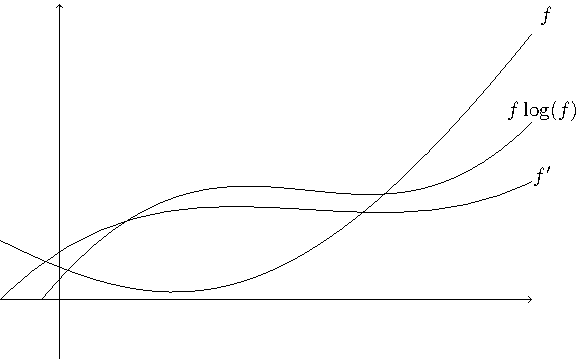
\includegraphics{./img/timespacehierarchies/timehierarchy.pdf}    
%        \caption{Affinché un linguaggio sia riconoscibile in $O(f)$ ma non in $O(f')$ richiediamo
%        che $f' \in o\left(\frac{f}{\log(f)}\right)$. Si congettura che questo gap logaritmico
%        ulteriore non sia necessario, ma ciò non è ancora stato dimostrato.}
%    \end{center}
%\end{figure}

Allo stato attuale della conoscenza non riusciamo ad essere più precisi al riguardo. Tuttavia non
è stato dimostrato che non si possa essere più precisi in questa classificazione. Questo però
non ci cambia molto dal punto di vista delle gerarchie: rimane l'inclusione stretta tra classi di
complessità come, ad esempio, $\DTIME(n)$ e $\DTIME(n^{2})$, e $\PClass$ e $\EXP$.

Anche in questo caso richiediamo la costruibilità in tempo della funzione che calcola il valore del
timer che fa da upper bound.

In tempo non riusciamo a fare classi così fini come riusciamo in spazio.

Abbiamo che se $f' \in o\left(\displaystyle\frac{f}{\log(f)}\right)$ allora abbiamo un linguaggio $\Lang$ riconoscibile in
tempo $O(f)$ ma non in tempo $O(f')$.

\section{Alcune gerarchie di complessità}

Definiamo alcune classi di complessità come segue:
\begin{itemize}
    \item $\PClass = \displaystyle\bigcup_{c \in \Nat}\DTIME(n^{c})$
    \item $\EXP = \displaystyle\bigcup_{c \in \Nat}\DTIME(2^{cn})$
    \item $\LOGSPACE = \DSPACE(\log)$
    \item $\PSPACE = \displaystyle\bigcup_{c \in \Nat}\DSPACE(n^{c})$
    \item $\EXPSPACE = \displaystyle\bigcup_{c \in \Nat}\DSPACE(2^{cn})$
\end{itemize}

Sappiamo che $\DTIME(2^{n})$ è diversa da $\DTIME(2^{2n})$, per il teorema della gerarchia in
tempo.  Un'altra possibile definizione di $\EXP$ è data dall'unione, su tutti i polinomi $p$, di
$\DTIME(2^{p})$. Sono due definizioni diverse, quest'ultima contiene la prima.

Abbiamo le seguenti relazioni tra queste classi di complessità:
\begin{itemize}
    \item $\LOGSPACE \subseteq \PClass \subseteq \PSPACE \subset \EXPSPACE$
    \item $\LOGSPACE \subset \PSPACE$
    \item $\PClass \subset \EXP \subseteq \EXPSPACE$
\end{itemize}

Per le inclusioni strette ci sono delle dimostrazioni, per quelle non strette non
sappiamo se siano strette.

Perché $\LOGSPACE$ è incluso in $\PClass$? I teoremi della gerarchia si applicano a classi uniformi di
complessità (spazio vs spazio, tempo vs tempo). Con $\PClass$ e $\LOGSPACE$ stiamo confrontando risorse
diverse, e perciò il teorema della gerarchia non si applica. Abbiamo che $\LOGSPACE$ contiene tutti
linguaggi riconoscibili in spazio $O(\log(n))$. Per il teorema tempo-spazio abbiamo che un
linguaggio con quella complessità in spazio è riconoscibile con una complessità in tempo
$O(2^{c\cdot(\log(n) + \log(n))}) = O(2^{c'\log(n)})$, per qualche $c'$. Ma $O(2^{c'\log(n)}) =
O(n^{c'})$, quindi abbiamo una complessità poliomiale in tempo, e quindi il nostro linguaggio fa
anche parte di $\PClass$.

\section{Padding}

Il padding è l'unica altra tecnica nota, oltre al teorema della gerarchia, per separare classi di
complessità.

Il padding è una trasformazione tra linguaggi. Abbiamo $\Lang$ e lo trasformiamo in $\LPad$.
Il linguagggio $\LPad$, ovvero il linguaggio delle stringhe paddate, è così definito:
\begin{equation*}
    \LPad = \set{x\#^{f(x)} \mid x \in \Lang}
\end{equation*}
A seconda della funzione $f$ cambia il padding.
\begin{equation*}
    x \mapsto x\overbrace{\#\#\cdots\#}^{f(x)}
\end{equation*}

L'obiettivo è ingrandire la dimensione delle stringhe del linguaggio. Possiamo fare qualunque tipo
di padding; di solito si fa un padding quadratico. È un'operazione di ``imballaggio'' delle
stringhe di $\Lang$ con un numero di simboli in più.

Ad esempio, se vogliamo un linguaggio con padding quadratico avremmo
\begin{equation*}
    \LPad = \set{x\#^{|x|^{2} - |x|} \mid x \in \Lang}
\end{equation*}

Supponiamo di avere $\Lang$ e $\LPad$. Qual è più semplice da riconoscere? $\LPad$. Per
riconoscere $\LPad$, ovvero decidere se una stringa paddata $w$ sta in $\LPad$, possiamo estrarre
$x$ da $w$ e verificare se $x \in \Lang$ con il riconoscitore di $\Lang$. La rimozione del padding
da $w$ ha costo lineare rispetto a $|w|$, è un'operazione semplice. Riconoscere $x$ ha una certa
complessità che dipende dalla dimensione di $x$. Tuttavia noi abbiamo ingrandito l'input: la
dimensione di $w$ è sicuramente maggiore di quella di $x$. Di conseguenza la complessità di
verificare se $w \in \LPad$, che calcoliamo rispetto alla dimensione di $w$, può essere minore
della complessità richiesta per verificare se $x \in \Lang$, a seconda del tipo di padding che
abbiamo fatto. 

Abbiamo questo fenomeno: gonfiando opportunamente l'input la complessità degli algoritmi sembra
diminuire.

Se ad esempio usiamo una notazione in base 1 per i numeri allora tutti gli algoritmi sembrano
migliorare drasticamente a livello di complessità. Ma questo miglioramento è fittizio, ed è
legato all'esplosione esponenziale della dimensione dell'input.

Tipicamente abbiamo uno speedup se calcoliamo la complessità del riconoscimento del linguaggio
paddato, proporzionale alla nuova dimensione dell'input.

Supponiamo, ad esempio, che la complessità richiesta per riconoscere $x$ sia $O(|x|^{2})$.
Supponiamo di fare un padding quadratico, ovvero di passare a $w$ con dimensione $|x|^{2}$. La
complessità dell'algoritmo di riconoscimento diventa $O(|w|)$, e sembra lineare. Tutto questo
discorso presuppone che estrarre $x$ da $w$ sia un'operazione di costo lineare in $|w|$.

\begin{figure}[h]
    \begin{center}
        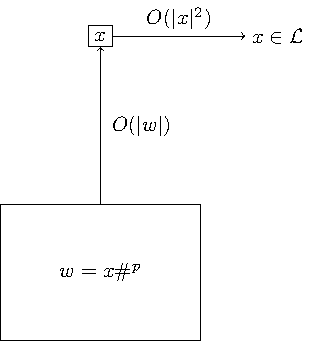
\includegraphics{./img/timespacehierarchies/PaddingSpeedup.pdf}    
        \caption{Riconoscere $\LPad$ costa in genere di meno di riconoscere $\Lang$}
    \end{center}
\end{figure}

Perché è interessante il padding? Perché ci può aiutare a separare classi di complessità. 

Supponiamo di avere due classi di complessità che vogliamo separare: $\CClass$ e $\CClass'$. Quando
vogliamo capire se due classi sono distinte ci possiamo chiedere rispetto a quali operazioni sono
chiuse.

Le trasformazioni prendono in input un linguaggio e ne restituiscono in output un altro. Che una
trasformazione produca un linguaggio all'interno della classe in cui si trovava il linguaggio di
input non è ovvio, e quando succede per ogni linguaggio della classe diciamo che la classe è
chiusa rispetto a questa trasformazione.

Un modo per separare le classi di complessità è prendere un'operazione, ad esempio il padding, e
verificare se una delle due è chiusa rispetto ad essa mentre l'altra non lo è. Con questo abbiamo
la dimostrazione che le due classi sono diverse.

\begin{figure}[h]
    \begin{center}
        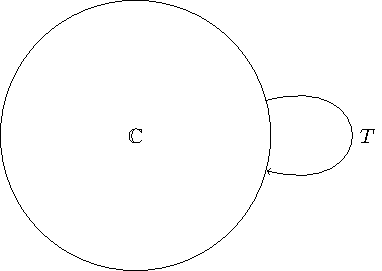
\includegraphics{./img/timespacehierarchies/ClosedClass.pdf}    
        \caption{La classe $\CClass$ in figura è chiusa rispetto alla trasformazione $T$}
    \end{center}
\end{figure}

Prendiamo $\PSPACE$ e $\EXP$. La nostra $\EXP$ e l'unione dei $\DTIME(2^{cn})$ per ogni $c \in
\Nat$. Si può definire $\EXP_{p}$ come l'unione di $\DTIME(2^{n^{c}})$ per ogni $c \in \Nat$. Sono
due classi diverse. Abbiamo che $\EXP \subset \EXP_{p}$: lo si dimostra con il teorema della
gerarchia.

Ci aspettiamo una relazione tra $\PSPACE$ ed $\EXP$? Sì. Per il teorema tempo spazio uno spazio
polinomiale implica un tempo esponenziale. Il grado dell'esponente, però, dipende dal polinomio.
Sicuramente $\PSPACE \subseteq \EXP_{p}$. Riusciamo a dimostrare altro? Non riusciamo a dimostrare
$\PSPACE \subset \EXP_{p}$ allo stato attuale dell'arte, anche se si suppone ciò. Si riesce a
dimostrare che $\PSPACE \not= \EXP$. Questo perché abbiamo che $\PSPACE$ è chiusa rispetto al
padding polinomiale, mentre $\EXP$ non lo è. Abbiamo inoltre che $\EXP_{p}$ è chiusa
rispetto ad un certo tipo di padding.

\begin{figure}[h]
    \begin{center}
        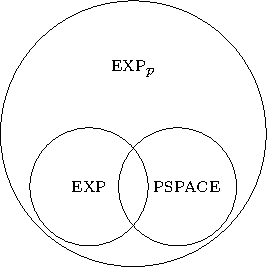
\includegraphics{./img/timespacehierarchies/ExpvsExppvsPSpace.pdf}
        \caption{Gerarchia congetturata tra le classi $\PSPACE$, $\EXP$ e $\EXP_{p}$}
    \end{center}
\end{figure}

\begin{thm}
    $\EXP \not= \PSPACE$
\end{thm}
\begin{proof}
    
    Dimostriamo innanzitutto che $\EXP \subset \DTIME(2^{n^{2}})$. Infatti abbiamo che $\forall c
    \in \Nat, 2^{cn} \in o(2^{n^{2}})$. L'unione di classi tutte contenute in $\DTIME(2^{n^{2}})$
    sta ancora in $\DTIME(2^{n^{2}})$. Dato che $\EXP$ è definita come il limite di questa unione
    potrebbe essere uguale a $2^{n^{2}}$, di conseguenza non ci basta l'ipotesi di prima per
    concludere $\EXP \subset \DTIME(2^{n^{2}})$. Ce ne serve una più forte: consideriamo
    $\DTIME(2^{n^{1.5}})$. Abbiamo che $\forall c,2^{cn} \in o(2^{n^{1.5}})$, e $\DTIME(2^{n^{1.5}})
    \subset \DTIME(2^{n^{2}})$ per il teorema della gerarchia. Di conseguenza $\EXP \subset
    \DTIME(2^{n^{2}})$

    Data questa inclusione stretta abbiamo che $\exists \Lang, \Lang \in \DTIME(2^{n^{2}}) \land
    \Lang \notin \EXP$. Consideriamo ora $\LPad$ con padding quadratico:
    \begin{equation*}
        \LPad = \set{ x\#^{|x|^{2}-|x|} \mid x \in \Lang}
    \end{equation*}

    Supponiamo per assurdo che $\PSPACE = \EXP$. Ci chiediamo ora, qual è la classe di complessità
    di $\LPad$? Di quanto decrescerà la complessità di riconoscere $\LPad$ rispetto alla
    complessità di riconoscere $\Lang$? Per riconoscere $\LPad$ noi partiamo da una stringa $w$ con
    una certa dimensione $|w|$. Da questa estraiamo, con complessità lineare, $x$, con lunghezza
    $n$ (da cui $|w| = n^{2}$). Cosa dobbiamo fare per verificare se $w \in \LPad$?  Dobbiamo
    verificare se $x \in \Lang$, con costo $O(2^{n^{2}})$. La complessità complessiva diventa
    $O(2^{|w|})$, ovvero con esponente lineare in $|w|$. Abbiamo quindi che $\LPad \in
    \DTIME(2^{n})$, il che implica che $\LPad \in \EXP$. Ma questo implica  $\LPad \in \PSPACE$ per
    la nostra ipotesi di assurdo.

    \begin{figure}[h]
        \begin{center}
            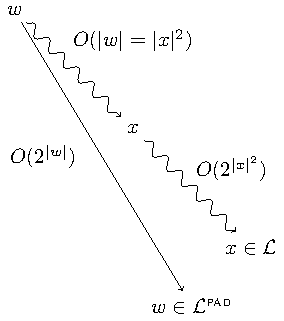
\includegraphics{./img/timespacehierarchies/PaddingCheat.pdf}
            \caption{Riconoscere $\LPad$ ha una complessità che ci permette di posizionarlo in
            $\EXP$ grazie al padding quadratico}
        \end{center}
    \end{figure}

    Cosa possiamo dire della complessità in tempo di riconoscere $\Lang$ sapendo che $\LPad \in
    \PSPACE$? Cosa dobbiamo fare per riconoscere $\Lang$ sotto questa ipotesi? Ci basta prendere
    $x$, paddarlo e darlo in pasto all'algoritmo di riconoscimento di $\LPad$. Il padding richiede
    tempo e spazio quadratico, e il riconoscimento di $\LPad$ lo facciamo in uno spazio polinomiale,
    poichè $\LPad \in \PSPACE$.

    \begin{figure}[h]
        \begin{center}
            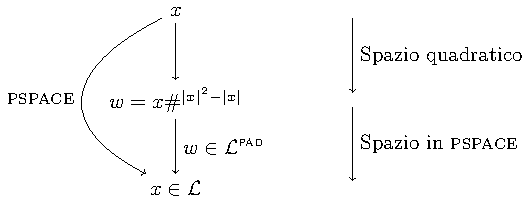
\includegraphics{./img/timespacehierarchies/LPadComplexity.pdf}
            \caption{Sapendo che $\LPad \in \PSPACE$ riusciamo a concludere che anche $\Lang$
            appartiene a $\PSPACE$}
        \end{center}
    \end{figure}

    Qua non possiamo fare il massimo tra le due operazioni per calcolare la complessità totale,
    dato che la stringa da cui partiamo è più piccola di quella paddata, e il padding ci costa.
    Ciò che conta però è che la composizione di polinomi è un polinomio, di conseguenza il
    processo usa uno spazio polinomiale.

    Di conseguenza $\LPad \in \PSPACE \implies \Lang \in \PSPACE \implies \Lang \in \EXP$, il che
    contraddice la nostra ipotesi iniziale.
\end{proof}

In questo caso abbiamo dimostrato che $\EXP \not= \PSPACE$ per assurdo. Si potrebbe anche dimostrare
facendo vedere che $\PSPACE$ è chiusa rispetto al padding polinomiale mentre $\EXP$ non lo è.

\subsection{Complessità della composizione di funzioni}

Sapendo qualcosa su due funzioni $f$ e $g$ sappiamo dire quanto ci costa calcolare $f(g(x))$? Non è
banale, perché noi misuriamo la complessità rispetto alla dimensione dell'input. Ci chiediamo quindi
prima quale sia l'ordine di grandezza degli output di $g$. Se lo sappiamo possiamo calcolare la
complessità di $f(g(x))$ usando la complessità di $f$, altrimenti no. Se gli output di $g$ fossero
costanti in dimensione non avrebbe neanche senso chiedersi quale sia la complessità di $f \circ g$,
dato che sarebbe sempre costante. A noi interessa la complessità di funzioni che prendono input che
possono crescere arbitrariamente.

Ad esempio, $g$ potrebbe produrre liste e $f$ potrebbe ordinarle. Supponiamo che $g$, data una
lista, produca il suo prodotto cartesiano. Supponiamo che $g$ non restituisca risultati ordinati.
Avremo un output di $g$ di dimensione $n^{2}$. In questo caso avremmo una complessità $O(n^{2} +
n^{2}\log(n^{2})) = O(n^{2}\log{n})$.

Se noi conosciamo solo la complessità in tempo possiamo dire qualcosa sulla dimensione degli
output? Con il teorema tempo spazio sappiamo che gli output prodotti sono bound dal tempo richiesto
dall'algoritmo. Non possiamo dare bound migliori per il caso pessimo.

\begin{figure}[!h]
    \begin{center}
        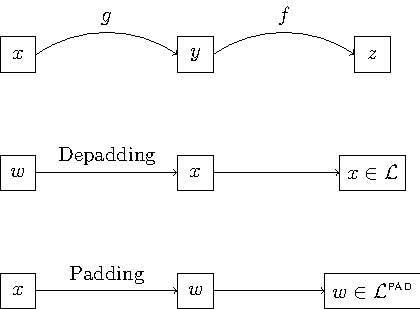
\includegraphics{./img/timespacehierarchies/FunctionsComposition.pdf}
        \caption{Per conoscere la complessità di $f \circ g$ dobbiamo conoscere l'ordine di
        grandezza degli output di $g$. Nel primo esempio abbiamo che l'output del depadding ha una
        dimensione pari alla radice quadrata dell'input, mentre il riconoscimento ha complessità
        $O(2^{|x|^{2}})$, per una complessità totale di $O(2^{|w|})$. Nel secondo esempio l'output
        del padding ha dimensione $O(|x|^{2})$, mentre il riconoscimento di $\LPad$ ha una
        complessità in $\PSPACE$, per una complessità totale in $\PSPACE$}
    \end{center}
\end{figure}

Bisogna stare attenti a capire se gli algoritmi producono strutture dimaniche. In tal caso c'è una
complicazione nel calcolo della complessità di una funzione composta. È un'analisi delicata.

\section{Conclusioni}

Volendo riassumere i risultati noti riguardanti le relazioni tra alcune classi di complessità
possiamo utilizzare un diagramma come quello in figura $\ref{timespacehierarchies:img:detclassesrelations}$. 

\begin{figure}[!h]
    \begin{center}
        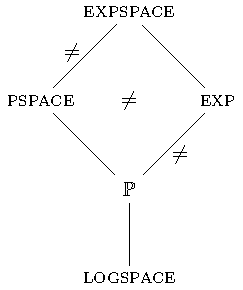
\includegraphics{./img/timespacehierarchies/ComplexityDiagram.pdf}
        \caption{Relazioni di inclusioni tra alcune classi di complessità}
        \label{timespacehierarchies:img:detclassesrelations}
    \end{center}
\end{figure}

Nel diagramma le linee vanno intese come inclusioni. Con il $\not=$ abbiamo un'inclusione stretta.

Se abbiamo a che fare con risorse dello stesso tipo possiamo usare il teorema della gerarchia per
dire qualcosa riguardo l'inclusione tra due classi di complessità.

Nel caso abbiamo a che fare con risorse di tipo diverso dobbiamo usare altri strumenti. Ad esempio
il teorema tempo spazio ci permette di stabilire inclusioni tra classi di complessità in tempo e
spazio.

Il teorema della gerarchia ci può dare inclusioni strette, quello tempo spazio dà solo inclusioni
lasche.

Il teorema tempo spazio ci dà, se abbiamo un bound polinomiale allo spazio, un bound esponenziale al
tempo di cui non conosciamo la costante.

Ad esempio, se abbiamo un algoritmo che lavora in spazio logaritmico abbiamo che lavorerà in tempo
polinomiale. Di questo polinomio però non possiamo sapere, in generale, il grado.

Nel parlare di classi ``feasible'', ovvero con complessità ragionevole, a volte si tende ad
escludere $\PClass$, perché risulta troppo grande, includendo problemi con complessità polinomiale
alta. Si preferisce quindi spesso restringersi a $\LOGSPACE$. In realtà anche questa non è ideale,
dato che ci possono essere algoritmi che lavorano in spazio logaritmico ma in tempo polinomiale con
un polinomio di grado alto. Inoltre esistono linguaggi riconoscibili in tempo polinomiale basso ma
che usano uno spazio più che logaritmico, che in questo caso vengono esclusi. In ogni caso
$\LOGSPACE$ resta una classe interessante che sta completamente in $\PClass$. Si congettura che
$\LOGSPACE \subset \PClass$, ma non si è ancora riusciti a dimostrarlo. 

$\PSPACE$ è molto più grande di $\NPClass$. Abbiamo infatti che $\PClass \subseteq \NPClass
\subseteq \PSPACE$, ma non si è ancora dimostrato $\PClass \not= \PSPACE$, nonostante lo si
congetturi.

Le inclusioni del diagramma che non sono strette sono inclusioni che sono congetturate essere
strette ma che non sono ancora state dimostrate esserlo. Le maggior parte delle inclusioni strette
vengono dai teoremi della gerarchia. La relazione tra $\EXP$ e $\PSPACE$ è invece dimostrabile
sfruttando il padding.

Il bound esponenziale dato dallo spazio al tempo è interessante perché, ad esempio, ci permette di
stabilire che $\LOGSPACE \subseteq \PClass$.
